\documentclass[12pt,a4paper]{article}
\usepackage{ssn-me-cse-review}
\usepackage{float}
\usepackage{url}
\usepackage{alltt}
\usepackage{longtable}
%\usepackage{mathtools}
\usepackage[document]{ragged2e}
\usepackage{algorithm2e}[1]
\usepackage{tikz}
\usetikzlibrary{shapes,arrows}
\usetikzlibrary{trees}
\newcommand{\comm}[1]{}
\usepackage{wasysym}
\begin{document}
\ptitle{Memotion Analysis : Automatic processing of Internet Memes}
\review{1}
\student{ Subalakshmi Shanthosi S (186001008)}
\semester{3}
\guide{Dr. Aravindan Chandrabose }
\reviewdate{14 August 2019}
\reviewtitle
\hrule

\section{Introduction}
In recent years, a huge amount of User Generated Content(UGC) online of various modalities like text,images and videos are accumulated on the web. NLP and Computer Vision communities often leverage only one prominent modality(text) in isolation to study social media.But,computational processing of internet meme needs a hybrid approach.This research work aims at building an automatic processing of Internet memes.

\section{Motivation}
Detection of offensive content on social media is an ongoing struggle due to the following reasons:\\
1. More number of emerging social websites creating voluminous data.\\Ex:Facebook,Flickr,Twitter,PinInterest etc. \\~\\
2. Prevalance of hate speech in social media is profound and it has become a great societal responsibility for the government and various social media companies to plan well ahead for mitigation and eventual prevention.\\~\\
3. Multimodal sentiment analysis is still in initial stage as it is less explored by many.\\~\\
\newpage
\subsection{Challenges in Memotion Analysis}:
1. A meme is uniquely multimodal as it has both visual and textual descriptors.\\
2. Most of the internet meme show replication in content by having same meme template with different sentences conveying same semantic meaning which are to be considered as duplicated in order to ensure better accuracy.\\~\\
3. Challenges in doing OCR compound when the number of potential fonts, languages, lexicons and other special characters increase.\\
Tesseract OCR isn't capable of handling italics and other special character encodings.\\
4.Defining correct visual descriptors which are to be evaluated in order to access the emotion is still a unanswered question.\\
5. Emotion Semantic Image Retrieval(ESIR) with affective gap
making the low-level image features extrapolate the high-level
semantics.
High-level features are nothing but textual descriptors like concept name, keywords etc.
Low-level features are qualitative measures of images like colour, texture, shape,spatial layout etc.
\section{Problem statement}
Memes typically induce humor and strive to be relatable. Some
memes are directly humorous whereas others go for sarcastic dig at
daily life events.Three subtasks varied by the degree of exploration
are as follows:\\~\\
1. \textbf{ Task A - Sentiment Classification}: Given an Internet meme, the first task is to classify it as positive or negative meme. We presume that a meme is not neutral.\\~\\
2. \textbf{ Task B- Humor Classification}: Given an Internet meme, the system has to identify the type of humor expressed. The categories are sarcastic, humorous, and offensive meme. If a meme does not fall under any of these categories, then it is marked as a other meme.\\~\\
3.\textbf{ Task C- Scales of Semantic Classes}: The third task is to quantify the extent to which a particular effect is being expressed(refer Table 1).
\newpage
8K human annotated Internet memes labelled with semantic dimensions namely sentiment, and type of humor that is, sarcastic, humorous, or offensive. 
\\~\\The humor types are further quantified on a likert scale as in Table 1. The dataset will also contain the extracted captions/texts from the memes.
\\~\\
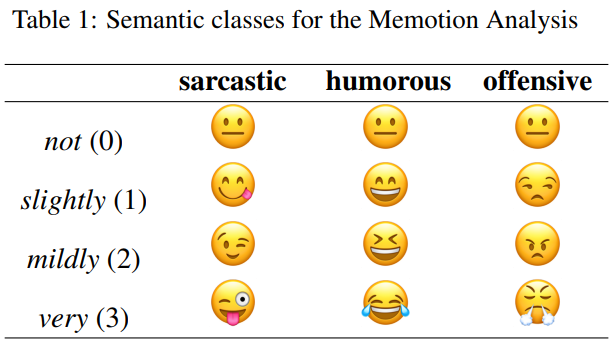
\includegraphics[scale=0.61]{semanticClass.png}
\section{Literature survey}
\subsection{Image-based memes as sentiment predictors\cite{imageSentimentPred}}
Opinion extraction by finding correlation between the implied semantic meaning of image-based memes and textual discussions in social media.Additionaly, trends in the use of popular memes are also identified. 
Visual predictors like colour,depth and shapes are used for image categorisation.\\
\textbf{Dataset Used}:\\
Facebook:Public posts and discussions.\\
10 discussion forums are taken into account with 997 unique
comments and 103 memes. A total of 27,260 words are existing.\\
Also for dynamic dataset Random discussions pages containing
memes are taken for processing.\\~\\
\newpage

\begin{table}[]
	\begin{tabular}{|l|l|}
		\hline
		\textbf{Category}                                                       & \textbf{Description}                                                                                                                                                                                                         \\ \hline
		\begin{tabular}[c]{@{}l@{}}Word \\ Analysis\end{tabular}       & \begin{tabular}[c]{@{}l@{}}Based on each words in a discussion.\\ Sentiment score calculated by using matching algorithm\\ to sentiment dictionary.\end{tabular}                                                    \\ \hline
		\begin{tabular}[c]{@{}l@{}}Phrase \\ Analysis\end{tabular}     & \begin{tabular}[c]{@{}l@{}}Semantria Sentiment Library to assign sentiment scores for\\ each phrase in the discussion.\\ Can also use phrase intensifiers like always or never.\end{tabular}                        \\ \hline
		\begin{tabular}[c]{@{}l@{}}Comment \\ Analysis\end{tabular}    & \begin{tabular}[c]{@{}l@{}}Averaged phrase analysis score for all the comments in\\ one discussion thread.\end{tabular}                                                                                             \\ \hline
		\begin{tabular}[c]{@{}l@{}}Discussion \\ Analysis\end{tabular} & \begin{tabular}[c]{@{}l@{}}Based on both word level and phrase level analysis.\\ Synonyms dictionary is constructed for "keyterm" and scores calculated by \\ comparing to find presence of that word.\end{tabular} \\ \hline
	\end{tabular}
	\caption{Textual Analysis of Facebook Discussions }
	\label{tab:my-table}
\end{table}
\begin{table}[]
	\begin{tabular}{|l|l|}
		\hline
		\textbf{Category}                                                                & \textbf{Description}                                                                                                                                                                                                                                                   \\ \hline
		\begin{tabular}[c]{@{}l@{}}Meme \\ Textual \\ Descriptions\end{tabular} & \begin{tabular}[c]{@{}l@{}}84\% memes are textual hence OCR extracted texts \\ are used for sentiment analysis.\\ Visual meme descriptors are found by finding appropriate action word \\ i.e) closest meaning word which describes that action.\end{tabular} \\ \hline
		\begin{tabular}[c]{@{}l@{}}Meme\\ Category\end{tabular}                 & \begin{tabular}[c]{@{}l@{}}Memes provided with categorical tag.\\ Tags:35,unique and descriptive entities\\ Ex:popcorn,teeth\end{tabular}                                                                                                                     \\ \hline
		\begin{tabular}[c]{@{}l@{}}Meme \\ Popularity\end{tabular}              & \begin{tabular}[c]{@{}l@{}}Frequency analysis of most common \\ meme category which where used.In addition to it existence of \\ particular tag is found on discussion forum as well.\end{tabular}                                                            \\ \hline
	\end{tabular}
	\caption{Meme Analysis }
	\label{tab:mytableTwo}
\end{table}
\textbf{Shortcomings}:\\
$\bullet$Misspelled words have NEUTRAL sentiment.\\
$\bullet$ Contradicting word-level and phrase level analysis.\\
\textbf{Future Work}:\\
$\bullet$ Sentiment dictionaries required addition of colloquial words or sensitive contextual words  like "banned" which have negative impact in Facebook but not found in sentiment dictionaries.\\
\newpage
\subsection{‘Meme’tic Engineering to Classify Twitter Lingo\cite{memeticEnggTwitter}}
Sentiment Analysis on textual memes is the main focus on this research work.Combination of Machine Learning and Image Processing Techniques to leverage maximal computation of meme emotion.\\~\\
\textbf{Datasets}:\\
1.Benchmark
Dataset:CSV file containing 1524 tweets labelled as:\\
\begin{itemize}
	\item POSITIVE(1)\\
	\item NEGATIVE(-1)\\
	\item NEUTRAL(0).
\end{itemize}
2.Dynamic Dataset using Twitter API:\\
Tweets gathered for a keyword given by the user.User login credentials are hashed and kept for finetuning dataset file inorder to login with those credentials to search for that keyword. \\~\\
\textbf{Machine Learning Techniques}:\\
\begin{itemize}
\item Multinomial Na\"ive Bayes Algorithm (Performant).\\
\item K-Nearest Neighbours(KNN) (More Performant).\\
\item Support Vector Machine(SVM) (Less Performant).\\
\item Logistic Regression(LR) (Moderate Performant).\\~\\
\end{itemize}
\textbf{Advantages}:\\
Efficient sentiment evaluator which can be
	easily integrated to enterprise applications.
KNN applicability even on small dataset.\\
\textbf{Shortcomings}:\\
Performance of OCR determines the accuracy of the system.
Visual descriptors are not given much attention for emotion evaluation.\\
\textbf{Future Work}:\\
Making the system multi-lingual and scaleble to volumnious data. 
\subsection{ Meme Opinion Categorization by Using Optical Character Recognition (OCR) and Na\"ive Bayes Algorithm\cite{memeOpinionOCR}}
This research work works on image-textual memes wherein the textual descriptor like comment/title phrases are extracted using Tesseract OCR.\\
Accuracy of OCR Tesseract is 75\%.\\
\textbf{Dataset}:\\
Meme Collection which specifically deals with viral memes about indonesian government.\\
Total Number of memes taken:100.\\
Randomly split in the ratio of 70\% and 30\% for training and testing respectively.\\
\textbf{Experimental Results}:
Na\"ive Bayes algorithm shows fairly good accuracy of 75\%.\\
Vmap tendency is calculated to find P\textsubscript{max} of all categories of
documents tested.\\
\textbf{Shortcomings}:\\
OCR less accurate:Inability to recognise italics.\\
OCR incapable of recognising special characters and emoticons.\\
\textbf{Future Work}:\\KNN,Neural network can be employed instead on Na\"ive Bayes as KNN could work on relatively smaller and low quality memes.
n-gram tokenisation for
enhanced preprocessing.
\subsection{ Rosetta: Large Scale System for Text Detection and Recognition in Images\cite{rosettaDataset}}
Rosetta is Facebook’s scalable OCR system.\\
Rosetta aims at becoming most scalable and robust OCR system capable of handling millions of requests per day.\\Two stage process:\\
Rosetta performs OCR in two independent steps:\\
\begin{enumerate}
	\item Detection of rectangular regions in the image potentially containing text.
	\item Text Recognition is performed on each detected regions using a CNN and then transcribe the word in the region.
\end{enumerate}
\newpage
\textbf{Text Detection Model}:\\
Approach based on Faster-RCNN a state-of-art object detection network.Faster-RCNN does detection and recognition simultaneously.\\
Supervised end-to-end process where each region's learning classifiers found (say k),which are sorted by their confidence score and non-maximum supression(NMS).
Alteration in Faster-RCNN - Replacement of ResNet convolutional body with a ShuffleNet-based architecture for improved efficiency.
\\The ShuffleNet convolutional body is pre-trained using ImageNet dataset.\\~\\
\textbf{Text Recognition Model}:\\
\begin{enumerate}
	\item  {\textbf{Character sequence encoding model(CHAR)}:\\
\textit{Assumption}:\\
$\bullet$ All images are of same size.\\
$\bullet$ Only k of it's characters are recognisable from a word regardless of the word length.\\
\textit{Working}:\\
The body of the CHAR model consists of a series of convolutions followed by k independent multiclass classification heads, each of which predicts the character of the alphabet (including the NULL character) at each position. During training, one jointly learns the convolutional body and the k different classifiers.}\\
\item {\textbf{Fully Conventional Model- CTC}:\\
	Known as CTC model because it uses sequence-to-sequence CTC loss during training.
	After convolutional body which is ResNet-18 , the last Convolutional layer predicts the most likely character at every image position of the input word.\\
	Example: LEARNING, the model might produce the sequence of characters "L-EE-A-RR-N-I-NN-G", which includes blanks and duplicates.\\
	\textit{Approach}:\\
	$\bullet$ Initialize the weights of the model body with the trained weights of the CHAR model, and then finetune those weights while simultaneously learning the last convolutional layer from scratch.\\
	$\bullet$The second approach was based on
	curriculum learning , i.e., starting with a simpler problem and increasing the difficulty as the model improves.Starting with word length 3 and gradually increasing them at every epoch.
}
\end{enumerate}
\newpage
\textbf{Datasets}:\\
1.COCO-Text which contains:
\begin{itemize}
	\item  63,000 images.
	\item  145,000 text instances.
\end{itemize}
2.Large synthetic dataset for covering maximum usecases as COCO-Text doesn't match the data-distribution of images uploaded to Facebook.
\begin{itemize} 
	\item 400k images for training.
	\item 50k images for testing.
\end{itemize}

\textbf{Experimental Results}:\\
Error rate of 37\% still recoverable by changing single character.\\
Finetuning with manually annotated corpus increased accuracy by 48.06\%\\
Random jitter introduced for data augmentation.\\
\textbf{Advantages}:\\
• Robust and accurate OCR capable of processing millions of
images per day.\\
• Faster search from TAO for recognised text.\\
• Adaptive character based recognition.\\

\textbf{Limitation}:\\
• Resolution of image increases inference time.\\
\textbf{Future Work}:\\
• Case sensitive labelling affected performance.\\

\subsection{An image-text consistency driven multimodal sentiment analysis approach for social media\cite{imageTextConsistency}}
•Visual feature detection using Local Binary Pattern.
• Textual Feature extraction: Continuous bag-of-words or skip-gram.
• Image-text similarity found.\\
\textbf{Datasets}: \\
• Visual Sentiment Ontology:\\
• Total number of images: 603.\\
• Topics:16.\\
\textbf{Training and Testing}:\\
• Training Dataset :400 images.\\
• Test Dataset: 157 images.\\
\newpage
\textbf{Results}:
•F-score:\\
• Positive
category:0.87
• Negative
category:0.89\\
• Adaptive merging of textual features with State-of-art
SentiBank for improved accuracy.\\
\textbf{Advantages}:\\
• Superior performance in Flickr benchmark dataset.\\
• Use of AdjectiveNounPair(ANP): Converting neutral noun
into Strong sentiment word.
\\\textbf{Shortcomings and Future Work}:\\
 • SVM modelling unrelated and related data sensitive to
outliers.\\
•ANP difficult due to it’s abstract nature and
high variability
\section{Existing system}
	 \begin{itemize}
	 	\item The existing approaches have used meme- discussion text correlation for finding concordance or using Pretrained CNN model for extracting top image content descriptors closet to the context. \cite{imageSentimentPred}\cite{imageTextConsistency}.
	 	\item Rosetta method of Extraction and pre-processing for additional data set creation can be done for multilingual memotion analysis\cite{rosettaDataset}
	 	\item KNN or Na\"ive Bayes classifier can be used for maximising F-score.\cite{memeOpinionOCR}\cite{memeticEnggTwitter} 	
	 \end{itemize}
 
\section{Proposed system}
  \begin{itemize}
  	\item Pre-trained CNN to work on either image or OCR extracted text classifier based on the image-text correlation.
  	\item Increasing working dataset size by using Rosetta Facebook's OCR system to make the system more generic by handling multiple languages.
  	\item KNN approach or Na\"ive Bayes classifier for opinion extraction to categorise as positive or negative.
  	\item Using ResNet for faster computation.
  \end{itemize}
\newpage
\begin{thebibliography}{99}
	\bibliographystyle{plain}
	
	\bibitem[1]{imageSentimentPred}Jean H. French, {\em Image-based Memes as Sentiment Predictors.
	}International Conference on Information Society (i-Society 2017).
	
	\bibitem[2]{memeticEnggTwitter}S. Priyashree, N. Shivani, D. K. Vigneshwar,S. Karthika, {\em International Conference on Computational Intelligence in Data Science(ICCIDS)}, 2017.
	\bibitem[3]{memeOpinionOCR}Amalia Amalia , Arner Sharif , Fikri Haisar , Dani Gunawan , Benny B Nasution ,{\em Meme Opinion Categorization by Using Optical Character Recognition (OCR) and Na\"ive Bayes Algorithm.} Third International Conference on Informatics and Computing (ICIC), 2018.
	\bibitem[4]{rosettaDataset} Bogdan Lazarescu, Christo Lolov , Silvia Sapora, {\em Rosetta: Large scale system for text detection and recognition in images.}, 
	KDD'18 Proceedings of the 24th ACM SIGKDD International Conference on Knowledge Discovery and Data Mining,Pages 71-79,2018.
	\bibitem[5]{imageTextConsistency}Ziyuan Zhao , Huiying Zhu , Zehao Xue and Zhao Liu  et al.,{\em An image-text consistency driven multimodal sentiment analysis approach for social media} , Information Processing and Management Vol 56-Issue 6,2019.
\end{thebibliography}
	
\end{document}
